% General layout
\pdfoutput=1
\documentclass[11pt]{article}
\usepackage[margin=1.0in]{geometry}

% Required packages
\usepackage{amsmath,amsfonts,amsthm,amssymb,mathrsfs} % Mathematical typesetting and symbols
\usepackage{enumerate} % Custom enumeration labels
\usepackage{fancyhdr} % Custom header and footer
\usepackage{graphicx} % Figure inclusion
\usepackage{hyperref} % Hyperlinks for citations, references, and URLs
\usepackage[numbers,sort&compress]{natbib} % Citation styling
\usepackage{subcaption} % Captions for subfigures
\usepackage{xcolor} % Text color

% Figure and table numbering by section
\counterwithin{figure}{section}
\counterwithin{table}{section}

% Theorem formatting for bold titles
\makeatletter
\def\th@plain{%
  \thm@notefont{}% same as heading font
  \itshape % body font
}
\def\th@definition{%
  \thm@notefont{}% same as heading font
  \normalfont % body font
}
\makeatother

% Theorem styles
\newtheorem*{definition}{Definition} % Definitions are not numbered
\newtheorem{theorem}{Theorem}[section] % Theorems numbered by section
\newtheorem{lemma}[theorem]{Lemma} % Lemma uses the same counter as Theorem
\newtheorem{observation}[theorem]{Observation} % Observation uses the same counter as Theorem
%\newtheorem{corollary}{Corollary}[theorem] % Corollary uses a sub-counter of Theorem
\newtheorem{corollary}[theorem]{Corollary} % Corollary uses the same counter as Theorem

% Custom Example environment
\theoremstyle{definition} % Examples are non-italicized
\newtheorem{ex}{Example}[section] % Examples are implemented as a type of Theorem
\newenvironment{example}[1][]{\begin{ex}[#1]}{\hfill$\blacksquare$\end{ex}} % Add a black box to the end automatically, and accept an optional title argument

% Course Definitions
\newcommand{\semesterlong}{Spring~2024}
\newcommand{\semestershort}{Sp24}
\newcommand{\courselong}{Optimization Theory}
\newcommand{\courseshort}{Optimization}
\newcommand{\coursecode}{MAP~4202}

% Overriding abbrvnat BibTeX template to use the plainurl template's DOI hyperlinks
\newcommand*{\doi}[1]{\href{https://doi.org/#1}{\tt doi:~#1}}

%==============================================================================

\title{Optimization Background}
% Note: Swapping the order of the author and date fields to exchange their order on the page.
\author{\coursecode:~\courselong\\\semesterlong}
\date{Adam Rumpf\footnote{Florida Polytechnic University, Department of Applied Mathematics, \href{mailto:arumpf@floridapoly.edu}{arumpf@floridapoly.edu}}}

%==============================================================================

\begin{document}

\maketitle

This set of introductory notes is meant to provide a brief summary of some fundamental concepts in mathematical optimization, and to review the optimization material that you should have seen in the calculus sequence. Our main textbook covers only \textit{linear} optimization, so for the first week or so of the course we will be relying on some of the off-book material in these notes to present optimization theory more broadly. Throughout the following, boldface variables~($\mathbf{x}$) will represent vector quantities while non-boldface variables~($x$) will represent scalar quantities.

%==============================================================================
\section{Mathematical Optimization in a Nutshell}
\label{sec:intro}

In mathematics, \textit{optimization} means more-or-less the same thing as it does in everyday speech: to \textit{optimize} a system means to adjust its inputs to produce the best possible output. To be more precise, mathematical optimization is about trying to find the inputs for a real-valued function (called the \textit{objective function}, or just the \textit{objective}) in order to achieve either the largest or the smallest value, possibly subject to some \textit{constraints} on the input variables.

Optimization problems arise all the time in real-world applications. Industrial engineers and operations researchers might be interested in making design decisions to minimize costs or maximize production capacity. Transportation engineers might want to make plans to minimize travel times or to maximize public transit coverage. Physicists might be interested in computing the outcome of a natural law that drives a system towards a minimum-energy or maximum-entropy state. Many models from statistics and machine learning are based on setting model parameters to minimize error or maximize likelihood given a set of training data. As long as we can describe the output of a system as a single, real objective value, then we can apply optimization theory to try to achieve the best possible outcome.

%%%
\subsection{The Structure of an Optimization Problem}
\label{subsec:structure}

A typical optimization problem is written in the form
\begin{alignat*}{3}
	\textrm{minimize} \quad& f(\mathbf{x}) &\qquad \text{or} \qquad&& \textrm{maximize} \quad& f(\mathbf{x}) \\
	\textrm{subject to} \quad& \mathbf{g}(\mathbf{x}) \le \mathbf{0} &&& \textrm{subject to} \quad& \mathbf{g}(\mathbf{x}) \le \mathbf{0}
\end{alignat*}

In the above examples, $f : \mathbb{R}^n \to \mathbb{R}$ is the \textbf{objective}, which is a function of the \textbf{decision variables} $\mathbf{x} \in \mathbb{R}^n$. The word ``minimize'' or ``maximize'' (usually abbreviated to just ``min'' or ``max'') is the \textbf{sense} of the optimization, and indicates whether our goal is to make the value of $f(\mathbf{x})$ as small or as large as possible.

Below the objective, after the words ``subject~to'' (usually abbreviated to just ``s.t.''), a set of \textbf{constraints} may be included (note that the boldface $\mathbf{g}$ and $\mathbf{0}$ indicate a \textit{vector} of inequalities to account for the possibility of having many constraints). Constraints can consist of sets of equalities and inequalities that the decision variables must satisfy (the above examples include $\le$ inequalities, but $\ge$ and $=$ are also allowed). Any decision vector $\mathbf{x}$ that satisfies all constraints is called a \textbf{feasible solution}, and the set of all feasible solutions is called the \textbf{feasible set}. Solving an optimization problem means finding the decision vector $\mathbf{x}$ that produces either the smallest (for minimization) or the largest (for maximization) objective value out of all solutions in the feasible set.

Sometimes variables may be listed underneath the ``min'' or ``max'' symbol to specify which variables represent the decisions. This is sometimes used to distinguish the decision variables from other parameters, or in more complicated optimization problems that contain multiple optimizations with respect to multiple sets of decision variables. Constraints may also be included there for brevity. As an example, assuming that it's clear from context that $x$ and $y$ are decision variables, the following four optimization problems are all equivalent.
\begin{alignat*}{7}
	\min \quad& x^2 y + 3y^2 &\hspace{0.5in}&& \min_{x,y} \quad& x^2 y + 3y^2 &\hspace{0.5in}&& \min_{x,y \ge 0} \quad& x^2 y + 3y^2 &\hspace{0.5in}&& \min \, \left\{ x^2 y + 3y^2 \, \middle| \, x,y \ge 0 \right\} \\
	\mathrm{s.t.} \quad& x,y \ge 0 &&& \mathrm{s.t.} \quad& x,y \ge 0
\end{alignat*}

%%%
\subsection{A Few Examples of Optimization Problem}
\label{subsec:examples}

We will end this section by showing a few examples of applied optimization problems.

\begin{example}
\label{ex:distance}
	Suppose we want to find the point $(x,y)$ on the graph of $y = x^2 - x$ that's closest to the point $(2,3)$. ``Closest'' means ``minimum distance'', so we can set this up as a minimization problem. The objective is the distance between $(x,y)$ and $(2,3)$, which is given by the Euclidean distance formula as
	\begin{align*}
		d = \sqrt{(x-2)^2 + (y-3)^2}
	\end{align*}
	while the constraint is that the point $(x,y)$ must lie on the graph of $y = x^2 - x$, which is true as long as $x$ and $y$ satisfy the equation $y = x^2 - x$. Then our optimization problem has the form
	\begin{align*}
		\min \quad& \sqrt{(x-2)^2 + (y-3)^2} \\
		\mathrm{s.t.} \quad& y = x^2 - x
	\end{align*}
	
	If we actually wanted to solve this, we could make things easier for ourselves by noting that the distance $d$ is minimized exactly when its square $d^2$ is minimized, so dropping the square root from the objective will still generate the same optimal solution, leaving the simpler optimization problem
	\begin{align*}
		\min \quad& (x-2)^2 + (y-3)^2 \\
		\mathrm{s.t.} \quad& y = x^2 - x
	\end{align*}
\end{example}

\begin{example}
\label{ex:factory}
	Suppose we're in charge of a furniture factory. There is ample demand and we can sell whatever products we manufacture, so the only constraints we need to consider arise from the limited amounts of material available. Suppose we can produce three different products: tables, chairs, and bookshelves. Manufacturing each product requires a different amount of wood (in pounds) and labor (in man hours), and each product sells for a different price. The attributes of each product are shown in Table~\ref{tab:furniture}.
	
	\begin{table}[h]
		\centering
		\begin{tabular}{l r r r}
			\hline Item & Wood (lbs) & Labor (h) & Price (\$) \\
			\hline Table & 275 & 4 & 600 \\
			Chair & 60 & 1.5 & 80 \\
			Bookshelf & 310 & 5 & 750 \\
			\hline
		\end{tabular}
		\caption{Material costs and selling prices of different furniture items.}
		\label{tab:furniture}
	\end{table}
	
	Suppose that we have 3000~lbs of wood and 200 man hours to work with. Our goal is to choose how many of each item to manufacture in order to maximize revenue while obeying the material limitations.
	
	Like most real-world problems, no variable names are given in the problem statement, so we will need to define our own. Let $t$ be the number of tables to produce, $c$ be the number of chairs, and $b$ be the number of bookshelves. Assuming that all produced items are sold, the revenue made from each item is just the number produced times the unit price, so the total revenue is
	\begin{align*}
		600t + 80c + 750b
	\end{align*}
	
	Likewise the amount of wood used for each item is the number produced times the wood cost, and the amount of labor used is the number produced times the labor cost. Limiting the total wood and labor usage to the amount of available material leads to constraints of the form
	\begin{align*}
		& 275t + 60c + 310b \le 3000 \\
		& 4t + 1.5c + 5b \le 200
	\end{align*}
	
	Finally, manufactured quantities obviously only make sense if they are nonnegative, so we should also include a nonnegativity constraint for each decision variable. This leads to an optimization problem of the form
	\begin{align*}
		\tag{maximize total revenue} \max \quad& 600t + 80c + 750b \\
		\tag{wood limitations} \mathrm{s.t.} \quad& 275t + 60c + 310b \le 3000 \\
		\tag{labor limitations} & 4t + 1.5c + 5b \le 200 \\
		\tag{nonnegativity} & t,c,b \ge 0
	\end{align*}
	
	If there is no carryover of projects in progress between manufacturing periods, then it might also make sense to require that $t$, $c$, and $b$ take integer values, however for reasons we will see later in the course it is desirable to avoid adding integer constraints whenever possible.
\end{example}

\begin{example}
\label{ex:leastsquares}
	A common application of optimization in statistics is \textit{model fitting}, wherein our goal is to design a model function (by setting its parameter values) in order to minimize the difference error between our model's predictions and the observed data. For example, suppose we have a set of observed input/output pairs of the form
	\begin{align*}
		(x_1,y_1), (x_2,y_2), \dots, (x_n,y_n)
	\end{align*}
	and that we have reason to believe there's a roughly linear relationship between the input $x$ and the output $y$. Then we might propose a model of the form
	\begin{align*}
		y(x) = mx + b
	\end{align*}
	for some choice of slope $m$ and intercept $b$. Our goal is to choose those parameters $m$ and $b$ in a way that minimizes the differences between the observed outputs $y_i$ and the predicted outputs $y(x_i)$ for $i=1,2,\dots,n$.
	
	The absolute error in our model's prediction for the $i$th observation is just the absolute difference between the two
	\begin{align*}
		|y_i - y(x_i)| = |y_i - mx_i - b|
	\end{align*}
	
	For various statistical and computational reasons, in practice it's common to measure our model's quality using the \textit{squared} error instead of the absolute error,
	\begin{align*}
		(y_i - y(x_i))^2 = (y_i - mx_i - b)^2
	\end{align*}
	
	The sum of squared errors over all data points provides a rough measurement of how close our model is to predicting the observed data. If we want the best possible model, we want to choose the parameters $m$ and $b$ that minimize the sum of squared errors, which leads to an optimization problem of the form
	\begin{align*}
		\min_{m,b} \quad& \sum_{i=1}^n (y_i - mx_i - b)^2
	\end{align*}
	subject to no constraints. This general structure of optimization problem appears all throughout statistical regression, but different measurements of error and different models $y(x)$ may be used depending on the application.
\end{example}

\begin{example}
\label{ex:knapsack}
	The \textit{knapsack problem} is a fundamental combinatorial optimization problem, and versions of it appear throughout operations research and computer science. The setup for the problem is this: Suppose we have a knapsack capable of holding a limited weight $K$. There is a collection of $n$ different items that we might want to bring with us on a camping trip, each having a given weight $w_i$ and value $v_i$. Our goal is to choose a subset of the items to pack into the knapsack, with the objective of maximizing the total value of all packed items, subject to the weight limit of the knapsack.
	
	Unlike the previous examples, the decisions being made here are binary: For each item, we either pack it or we don't, with no possibility in between. This provides a hint for how we might formulate the knapsack problem as a mathematical program. For each item $i=1,2,\dots,n$, we can define a decision variable $x_i$ which is allowed to take only two possible values: $1$~to represent the decision to pack the item, or $0$~to represent the decision to leave the item. In this way each variable $x_i$ can be used like a boolean variable (yes/no, true/false, etc.) from a computer program.
	
	With these decision variables defined, the value we gain from item $i$ is simply the product $v_i x_i$ (zero if we don't take it, and $v_i$ if we do) while the weight of the item in the knapsack is $w_i x_i$ (zero if we don't take it, and $w_i$ if we do). Then we can formulate the knapsack problem as
	\begin{alignat*}{2}
		\tag{maximize total value} \max \quad& \sum_{i=1}^n v_i x_i \\
		\tag{weight limit} \mathrm{s.t.} \quad& \sum_{i=1}^n w_i x_i \le K \\
		\tag{binary decisions} & x_i \in \{0,1\} &\qquad& i=1,2,\dots,n
	\end{alignat*}
\end{example}

\begin{example}
\label{ex:networkdesign}
	Consider a road network engineering problem concerning the road network displayed in Figure~\ref{fig:networkdesign}. The numbered dots $1,2,\dots,6$ represent traffic intersections while the arrows between the dots represent segments of road, with the direction of the arrow indicating the direction of traffic.
	
	\begin{figure}[h]
		\centering
		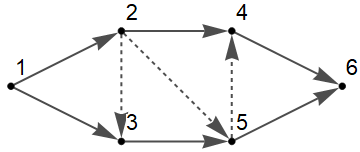
\includegraphics[width=0.4\textwidth]{figures/network_design_01.png}
		\caption{A road network. Solid arrows represent existing roads, while the dashed arrows represent new roads that can be built. Traffic must get from $1$ to $6$ while obeying the directions of the arrows.}
		\label{fig:networkdesign}
	\end{figure}
	
	Suppose our goal is to get 500 units of traffic from intersection 1 to intersection 6 while minimizing the total driving time of all users. Part of that task can be accomplished by choosing how to route traffic through the network\footnote{Of course, in practice, the transportation planner does not control divers directly. In most real-world road network engineering we need to apply game theoretic models for user behavior, which generally assume that each individual driver is attempting to minimize their own personal travel time. This tends to lead to very different behavior than what we would see if we could control traffic patterns directly, and also leads to some strange apparent paradoxes, like the opening of new roads actually making overall travel times worse. We're ignoring that for now.}, but suppose we are also allowed to build \textit{one} additional road segment to help to help with the flow of traffic. The three candidate locations for the new road segment are marked by the dashed arrows.
	
	Making these plans requires some additional information about the network. Consider any pair of adjacent intersections $i$ and $j$ connected by a road segment, which we will simply call road $ij$. Suppose that, under normal operating conditions, it takes $t_{ij}$ minutes\footnote{In practice we also usually include congestion models to account for travel time of a road increasing as more people use it. We're ignoring that here, as well.} to drive from $i$ to $j$, and that a maximum of $c_{ij}$ units of traffic can be carried by road $ij$ (the $ij$ subscripts for $t_{ij}$ and $c_{ij}$ indicate that the time and capacity could be different for each road segment $ij$). 500 units of traffic begin at intersection 1 and are destined for intersection 6. Assume that no other traffic enters or leaves the network.
	
	There are two types of decisions to be made here: which available road (23, 25, or 54), if any, should be built, and how should the traffic be routed through the resulting network. As a result, we will introduce two different types of decision variable: continuous variables $x_{ij}$ to represent the amount of traffic to send through each road $ij$, and binary variables $z_{ij}$ for each of the three available new roads, to be set equal to 1 if we decide to build the road and 0 otherwise.
	
	The total time that users spend driving on road $ij$ is $t_{ij} x_{ij}$. Summing this over all nine roads in the network gives the total user travel time as
	\begin{align*}
		t_{12} x_{12} + t_{13} x_{13} + t_{23} x_{23} + t_{24} x_{24} + t_{25} x_{25} + t_{35} x_{35} + t_{46} x_{46} + t_{54} x_{54} + t_{56} x_{56}
	\end{align*}
	
	We know that 500 units of traffic must leave intersection 1. There are only two roads, $12$ and $13$, that exit intersection 1, so we have the constraint
	\begin{align*}
		500 = x_{12} + x_{13}
	\end{align*}
	
	Similarly, 500 units must enter intersection 6, so we also have the constraint
	\begin{align*}
		x_{46} + x_{56} = 500
	\end{align*}
	
	As for the intermediate intersections, every car that enters an intersection via one road must leave it through another road. Then we should have a \textit{flow conservation} constraint for each intersection to enforce the fact that inflow must equal outflow. Taking intersection 5 as an example, setting inflow equal to outflow gives us
	\begin{align*}
		x_{25} + x_{35} = x_{54} + x_{56}
	\end{align*}
	
	Each road has a limited capacity, which allows us to place an upper bound on each of the traffic flow variables $x_{ij}$. To respect the directions of the roads we should also require that the flows be nonnegative, so for each road $ij$ we should have constraints
	\begin{align*}
		0 \le x_{ij} \le c_{ij}
	\end{align*}
	
	Finally, to account for the construction projects, we are allowed to build at most one new road, which means that at most one of the three construction decision variables $z_{23}$, $z_{25}$, and $z_{54}$ variables should be 1. This can be easily enforced by just bounding their sum by 1
	\begin{align*}
		z_{23} + z_{25} + z_{54} \le 1
	\end{align*}
	
	We also need a way for the construction decisions to actually affect the traffic flow variables $x_{ij}$, since we should not be able to use a road that has not been built. For example, if we decide to build road $23$ by setting $z_{23} = 1$, then traffic flow should be allowed on road $23$ up to its capacity, in which case $x_{23} \le c_{23}$. If we decide not to by setting $z_{23} = 0$, then no traffic should be allowed on road $23$ and we should force $x_{23} = 0$. This relationship can be enforced by a constraint of the form
	\begin{align*}
		0 \le x_{23} \le c_{23} z_{23}
	\end{align*}
	
	Putting everything together, we arrive at an optimization problem of the form
	\begin{align*}
		\tag{minimize total driving time across all roads} \min \quad& t_{12} x_{12} + t_{13} x_{13} + t_{23} x_{23} + t_{24} x_{24} + t_{25} x_{25} + t_{35} x_{35} + t_{46} x_{46} + t_{54} x_{54} + t_{56} x_{56} \\
		\tag{inflow = outflow at intersection 1} \mathrm{s.t.} \quad& 500 = x_{12} + x_{13} \\
		\tag{inflow = outflow at intersection 2} & x_{12} = x_{23} + x_{25} + x_{24} \\
		\tag{inflow = outflow at intersection 3} & x_{13} + x_{23} = x_{35} \\
		\tag{inflow = outflow at intersection 4} & x_{24} + x_{54} = x_{46} \\
		\tag{inflow = outflow at intersection 5} & x_{25} + x_{35} = x_{54} + x_{56} \\
		\tag{inflow = outflow at intersection 6} & x_{46} + x_{56} = 500 \\
		\tag{capacity of road $12$} & 0 \le x_{12} \le c_{12} \\
		\tag{capacity of road $13$} & 0 \le x_{13} \le c_{13} \\
		\tag{capacity of road $24$} & 0 \le x_{24} \le c_{24} \\
		\tag{capacity of road $35$} & 0 \le x_{35} \le c_{35} \\
		\tag{capacity of road $46$} & 0 \le x_{46} \le c_{46} \\
		\tag{capacity of road $56$} & 0 \le x_{56} \le c_{56} \\
		\tag{capacity and construction of road $23$} & 0 \le x_{23} \le c_{23} z_{23} \\
		\tag{capacity and construction of road $25$} & 0 \le x_{25} \le c_{25} z_{25} \\
		\tag{capacity and construction of road $54$} & 0 \le x_{54} \le c_{54} z_{54} \\
		\tag{limit construction to 1 road} & z_{23} + z_{25} + z_{54} \le 1 \\
		\tag{binary construction decisions} & z_{23}, z_{25}, z_{54} \in \{0,1\}
	\end{align*}
\end{example}

\newpage
%==============================================================================
\section{Properties of an Optimization Problem}
\label{sec:properties}

Mathematical optimization is an exceptionally broad and varied field due to the fact that different types of optimization problems with different mathematical properties may require fundamentally different solution approaches arising from fundamentally different branches of mathematics. More specifically, the properties of the objective function and the feasible set determine the types of solution techniques that may be required. A big part of working with optimization-based models revolves around formulating a model and then deciding on an appropriate solution strategy based on the properties of that model, or potentially reformulating and simplifying the model to make it easier to solve.

There are many, \textit{many} branches of optimization theory and many different relevant properties that an optimization problem can possess. A few of the broad distinctions that will be important in this course are explained below, but throughout the course we will see more structural properties that can be taken advantage of to develop specialized solution algorithms.

%%%
\subsection{Constrained versus Unconstrained Optimization}
\label{subsec:constrained}

An optimization problem that does not include any constraints is called \textbf{unconstrained}; otherwise it is \textbf{constrained}. Constraints generally make the problem harder by placing restrictions on the feasible set, and optimization techniques for constrained problems are generally more complicated than those for unconstrained problems. That being said, unconstrained problems are still common enough in applications (especially statistics and machine learning) that it is useful to develop algorithms specifically for them. We will be dealing primarily with unconstrained problems when we discuss nonlinear optimization near the end of this course.

%%%
\subsection{Discrete versus Continuous Optimization}
\label{subsec:integer}

In many situations there is good reason for some decision variables to be restricted to take integer values. For example, if one decision represents a number of cars to build, a fractional result would not make sense. Moreover, many decisions are naturally binary (yes/no), and it is common to model them using a binary decision variable required to take values in the set $\{0,1\}$, as seen in Examples~\ref{ex:knapsack} and~\ref{ex:networkdesign}. More generally, this type of binary indicator variable is often used (in potentially complicated ways) to enforce logical constraints.

An optimization problem that includes integer variables is called an \textbf{integer program (IP)}. Integer programs are generally far more difficult to solve than non-integer programs, and no efficient algorithms are known for solving general integer programs exactly, so most of the solution techniques used in practice have to resort to approximation. We will discuss integer programs between our coverage of linear and nonlinear programs near the middle of this course.

%%%
\subsection{Linear versus Nonlinear Optimization}
\label{subsec:nonlinear}

A \textbf{linear program (LP)} is an optimization problem for which the objective function and all constraint functions are \textit{affine}; that is, they consist of linear combinations of the decision variables plus constants. For example,
\begin{alignat*}{5}
	\min &\quad& 3x &\,+\,& 4y &\,-\,& z \\
	\mathrm{s.t.} && x &\,-\,& 2y &\,+\,& 5z &\,=\,& 7 \\
	&& 2x &\,+\,& 3y &\,+\,& 2z &\,=\,& 4 \\
	&& && y &\,+\,& z &\,\ge\,& 0
\end{alignat*}
is a linear program since the objective and constraint functions are all affine. Example~\ref{ex:factory} in the previous section was linear. Example~\ref{ex:networkdesign} was what is known as a \textbf{mixed integer/linear program (MILP)}, which is a linear program containing a mixture of continuous and integer variables.

An optimization problem is called a \textbf{nonlinear program (NLP)} if it has a non-affine objective or any non-affine constraints. For example,
\begin{alignat*}{5}
	\max &\quad& 2x &\,+\,& x^2 &\,+\,& y \\
	\mathrm{s.t.} && 5x &\,-\,& 3x^2 &\,+\,& 3y &\,\ge\,& 2 \\
	&& && x &\,-\,& y &\,=\,& 1
\end{alignat*}
is a nonlinear program since it includes powers of a decision variable ($x^2$). Examples~\ref{ex:distance} and~\ref{ex:leastsquares} were nonlinear programs. The majority of this course will be spent studying linear programs, and we will move on to see a few techniques for nonlinear programs near the end of the course.

%%%
\subsection{Convex versus Nonconvex Optimization}
\label{subsec:convex}

A \textbf{convex program} is a minimization problem for which the objective function and feasible set are both \textit{convex}. Convex programs appear naturally in a wide variety of contexts, and they have some ``nice'' properties that make them easier than most general optimization problems to solve. Most nonlinear problems are not convex, but all linear programs are convex, which is one of the properties that will allow us to come up with efficient LP solution algorithms later in the course.

We will study convex programs in more detail after we begin our discussion of nonlinear optimization, but for now it's enough to have a simple, visual understanding of what it means for a set or a function to be convex. A \textbf{convex set} $S \subseteq \mathbb{R}^n$, roughly speaking, is one that consists of a single contiguous region with no holes or divots (see Figure~\ref{fig:convexset}). A \textbf{convex function} $f : \mathbb{R}^n \to \mathbb{R}$, roughly speaking, is one whose graph is bowl-shaped (see Figure~\ref{fig:convexfunction}). See \textit{Convex Optimization}~\cite{boyd} for more details.

\begin{figure}[h]
	\centering
	
	\begin{subfigure}{0.4\textwidth}
		\centering
		
\includegraphics[width=0.4\textwidth]{figures/convexset01.png} 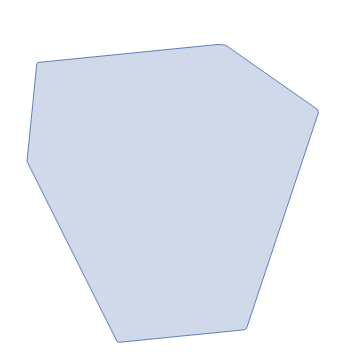
\includegraphics[width=0.4\textwidth]{figures/convexset02.png}
		\caption{Convex sets.}
	\end{subfigure}
	\hfill
	\begin{subfigure}{0.575\textwidth}
		\centering
		
\includegraphics[width=0.275\textwidth]{figures/nonconvexset01.png} 
\includegraphics[width=0.275\textwidth]{figures/nonconvexset02.png} 
\includegraphics[width=0.275\textwidth]{figures/nonconvexset03.png}
		\caption{Nonconvex sets.}
	\end{subfigure}
	
	\caption{Examples of convex and nonconvex sets $S \subset \mathbb{R}^2$.}
	\label{fig:convexset}
\end{figure}

\begin{figure}[h]
	\centering
	
	\begin{subfigure}{0.45\textwidth}
		\centering
		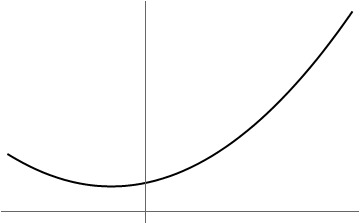
\includegraphics[width=0.45\textwidth]{figures/convexfunction01.png} \quad 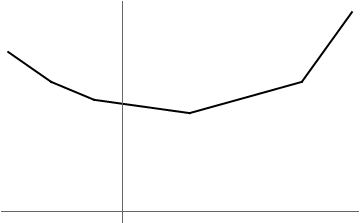
\includegraphics[width=0.45\textwidth]{figures/convexfunction02.png}
		\caption{Convex functions.}
	\end{subfigure}
	\hfill
	\begin{subfigure}{0.45\textwidth}
		\centering
		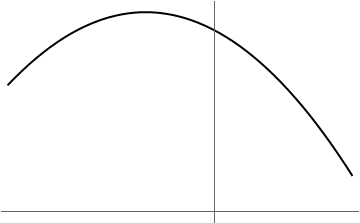
\includegraphics[width=0.45\textwidth]{figures/nonconvexfunction01.png} \quad 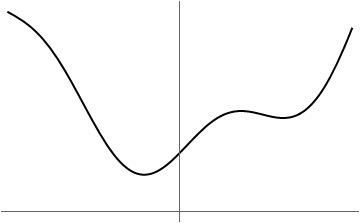
\includegraphics[width=0.45\textwidth]{figures/nonconvexfunction02.png}
		\caption{Nonconvex functions.}
	\end{subfigure}
	
	\caption{Examples of convex and nonconvex functions $f : \mathbb{R} \to \mathbb{R}$.}
	\label{fig:convexfunction}
\end{figure}

The main important property of convex programs that will be useful to us in this course is the fact that, for a convex function defined on a convex set, a solution is a \textit{local minimum} if and only if it is a \textit{global minimum} (local and global minimums will be defined precisely in the next section). We will see the proof for this result later in the course, but for now you can probably visualize why it must be true based on the shape of a convex function's graph. This is a useful property because, as we will soon see, it is relatively easy to design algorithms to search for local minima, and in the case of convex programs those algorithms can also find the global minimum.

Finally, the negative of a convex function is called a \textbf{concave function}. Roughly speaking, it is a function whose graph is dome-shaped (an example of this can be seen in the left graph of Figure~\ref{fig:convexfunction}b). In the same way that a local minimum of a convex function must be a global minimum, a local \textit{maximum} of a \textit{concave} function must be a global \textit{maximum} (you can probably convince yourself graphically why this must be true). For this reason, in optimization, we generally consider \textit{convex minimization} and \textit{concave maximization} to be ``easy'' problems, relatively speaking.

\newpage
%==============================================================================
\section{Review of Optimization in Calculus}
\label{sec:calculus}

Optimization is one of the major applications of differential calculus typically discussed in Calculus~I and Calculus~III. In this section we will briefly review this approach to optimization, which revolves around the principle of \textit{critical points}. Most of this should be a review for you, but we will define and prove things with a bit more precision than you might have gone over when you first went through the Calculus sequence. See Stewart's \textit{Calculus}~\cite{stewart} (which some of you may very well still own) or OpenStax \textit{Calculus}~\cite{openstax1,openstax3} (which is available for free online) for more details. See also Appendix~\ref{app:partial} for a review of partial derivatives and the gradient vector.

%%%
\subsection{Local and Global Optima}
\label{subsec:localglobal}

\begin{figure}[h]
	\centering
	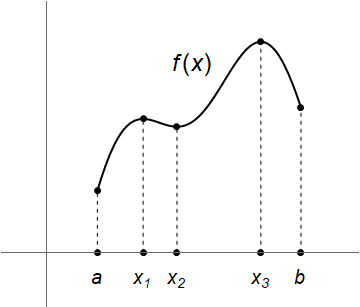
\includegraphics[height=0.225\textheight]{figures/local_extrema.png}
	\caption{A continuous function $f : [a,b] \to \mathbb{R}$ with several local minima and maxima.}
	\label{fig:localextrema}
\end{figure}

Figure~\ref{fig:localextrema} shows the graph of a generic function $f : [a,b] \to \mathbb{R}$ that might typically be studied during the optimization sections of a Calculus~I course. The graph includes several peaks and valleys, and our goal in minimizing or maximizing $f$ on the domain $[a,b]$ is intuitively to find the lowest or the highest point on the graph. In the case of a simple function of one variable it's easy enough for us to look at its graph to immediately see the minimum and maximum values, but in order to deal with functions of many variables we'll need to develop some more general definitions and terminology, starting with the distinction between \textit{local} and \textit{global} optima.

\begin{definition}[Local Optimum]
	Let $f : D \to \mathbb{R}$ be a real-valued function defined on a set~\mbox{$D \subseteq \mathbb{R}^n$}. An input $\mathbf{a}$ is called a \textbf{local minimizer} of $f$ if
	\begin{align*}
		f(\mathbf{a}) \le f(\mathbf{x})
	\end{align*}
	for all $\mathbf{x}$ in some ball centered at $\mathbf{a}$. Similarly, an input $\mathbf{b}$ is called a \textbf{local maximizer} of $f$ if
	\begin{align*}
		f(\mathbf{b}) \ge f(\mathbf{x})
	\end{align*}
	for all $\mathbf{x}$ in some ball centered at $\mathbf{b}$.
\end{definition}

In short, a point is a local minimum if its function value is smaller than all ``nearby'' function values, and it is a global maximum if its function value is larger. The precise definition of ``nearby'' depends on the function and the point, but it should always be possible to find a small enough nonzero radius for the local minimum (maximum) to have smaller (larger) function value than everything else within that radius. In Figure~\ref{fig:localextrema} we can see that $a$, $x_2$, and $b$ are all locally minimal while $x_1$ and $x_3$ are all locally maximal. This leads to the closely-related definition of a \textit{global} optimum.

\begin{definition}[Global Optimum]
	Let $f : D \to \mathbb{R}$ be a real-valued function defined on a set~\mbox{$D \subseteq \mathbb{R}^n$}. A point $\mathbf{a}$ is called a \textbf{global minimizer} of $f$ if
	\begin{align*}
		f(\mathbf{a}) \le f(\mathbf{x})
	\end{align*}
	for all $\mathbf{x} \in D$. Similarly, a point $\mathbf{b}$ is called a \textbf{global maximizer} of $f$ if
	\begin{align*}
		f(\mathbf{b}) \ge f(\mathbf{x})
	\end{align*}
	for all $\mathbf{x} \in D$.
\end{definition}

In short, a point is a global minimum if its function value is smaller than any other on the entire domain of the function, and it is a global maximum if its function value is larger. The global optima are what we're really looking for when we solve optimization problems. In Figure~\ref{fig:localextrema} we can see that $a$ is the global minimum while $x_3$ is the global maximum.

It might not be immediately obvious, but it's possible to have a function defined on a domain for which no global minimum or maximum exists. This would be problematic if we wanted to optimize such a function, since it would mean that the associated optimization problem would have no solution. Fortunately there are some fairly easy sufficient conditions for the existence of global optima.

\begin{theorem}[The Extreme Value Theorem]
\label{thm:extreme}
	Let $f : D \to \mathbb{R}$ be a continuous, real-valued function defined on a closed and bounded set~$D \subset \mathbb{R}^n$. Then~$f$ must attain its absolute maximum and minimum values on~$D$, meaning that there must exist points~$\mathbf{a}, \mathbf{b} \in D$ such that
	\begin{align*}
		f(\mathbf{a}) \le f(\mathbf{x}) \le f(\mathbf{b})
	\end{align*}
	for all $\mathbf{x} \in D$.
\end{theorem}

Proving the Extreme Value Theorem is beyond the scope of this course and requires some advanced functional analysis\footnote{If you're interested in the details, see the first chapter of Hunter and Nachtergaele's \textit{Applied Analysis}~\cite{hunter}, which is available for free online.}. The Extreme Value Theorem is a foundational result in optimization theory since it provides a very simple set of criteria to guarantee the existence of a global minimum and maximum, without which there wouldn't be much point in trying to optimize a function in the first place. Most of the functions and domains that we will examine in this class are cases for which the Extreme Value Theorem applies, however we will deal with many cases for which the feasible set is unbounded (in particular, this is always the case in unconstrained optimization), in which case the objective value may also be unbounded.

%%%
\subsection{Critical Points}
\label{subsec:critical}

From Figure~\ref{fig:localextrema} we can see that, for a continuous function $f$, one of the things we should expect to be true at a local optimum $c$ is that the slope of the graph be zero, meaning that $f'(c)$ should be zero. This makes intuitive sense, since if $f'(c)$ were positive the value of $f$ would be greater than $f(c)$ just to the right of $c$ and less than $f(c)$ just to the left of $c$, both of which would contradict $f(c)$ being locally optimal. A similar situation would occur if $f'(c)$ were negative.

This requirement that the derivative of a differentiable function be zero at a local optimum is sometimes called \textbf{stationarity}: As we pass through a local maximum or minimum, the value of the function should become momentarily \textit{stationary}, neither increasing nor decreasing, which is what happens at a peak or a valley. This intuitive requirement is captured more precisely by \textit{Fermat's Theorem}\footnote{Not the famous Fermat's \textit{Last} Theorem, or the slightly less famous Fermat's \textit{Little} Theorem.}.

\begin{theorem}[Fermat's Theorem]
\label{thm:fermat}
	Let $f : I \to \mathbb{R}$ be a real-valued function defined on some open interval $I \subseteq \mathbb{R}$. If $c$ is a local optimum of $f$ and $f$ is differentiable at $c$, then $f'(c) = 0$.
\end{theorem}

\begin{proof}
	Suppose that $f$ has a local optimum at $c$ and that $f$ is differentiable at $c$. We will assume that $f(c)$ is a local minimum of $f$, since the case of a local maximum can be handled analogously.
	
	Since $f$ is differentiable at $c$, the limit
	\begin{align*}
		f'(c) = \lim_{x \to c} \frac{f(x) - f(c)}{x - c}
	\end{align*}
	must exist. This implies that both one-sided limits also exist and are equal to the overall limit, so
	\begin{align}
		\label{eqn:fermat1} \lim_{x \to c^+} \frac{f(x) - f(c)}{x - c} = \lim_{x \to c} \frac{f(x) - f(c)}{x - c} = f'(c)
	\end{align}
	
	Since $f(c)$ is a local minimum of $f$, the numerator $f(x) - f(c)$ is nonnegative for all $x$ within some neighborhood around $c$. In addition, in the right-handed limit, $x - c$ must be strictly positive as $x \to c^+$. Therefore the entire lefthand side of~(\ref{eqn:fermat1}) is nonnegative, and we can say that $f'(c) \ge 0$.
	
	On the other hand, we also have
	\begin{align}
		\label{eqn:fermat2} \lim_{x \to c^-} \frac{f(x) - f(c)}{x - c} = \lim_{x \to c} \frac{f(x) - f(c)}{x - c} = f'(c)
	\end{align}
	
	In the left-handed limit, $x - c$ must be nonpositive as $x \to c^-$. Therefore the entire lefthand side of~(\ref{eqn:fermat2}) is strictly negative, and we can say that $f'(c) \le 0$. Combining the two results $f'(c) \ge 0$ and $f'(c) \le 0$, we can conclude that $f'(c) = 0$.
\end{proof}

Note that Fermat's Theorem only implies that the derivative of the function be zero as long as it's differentiable at an extreme point, and as long as the extreme point occurs within an open interval. Since the Theorem makes no claims about what happens at non-differentiable points and on the boundaries of closed sets, we can immediately come up with a useful corollary for characterizing candidate extrema.

\begin{corollary}
\label{cor:fermat}
	Let $f : I \to \mathbb{R}$ be a real-valued function defined on some interval $I \subseteq \mathbb{R}$. If $c$ is a local optimum of $f$, then at least one of the following must be true:
	\begin{enumerate}[(a)]
		\item $f'(c) = 0$
		\item $f'(c)$ is undefined
		\item $c$ is on the boundary of $I$
	\end{enumerate}
\end{corollary}

In order to simultaneously capture all of these possibilities in a single definition, we define a \textit{critical number} of a function.

\begin{definition}[Critical Number]
	Let $f : (a,b) \to \mathbb{R}$ be a real-valued function. A number $c \in (a,b)$ is called a \textbf{critical number} of $f$ if $f'(c)$ is either zero or undefined.
\end{definition}

Note that a function cannot be differentiable if it is discontinuous, so critical points include points of discontinuity as well as cusps. See Figure~\ref{fig:critical} for illustrations of different types of critical points, some of which correspond to local extrema and some of which do not.

\begin{figure}[h]
	\centering
	
	\begin{subfigure}{0.3\textwidth}
		\centering
		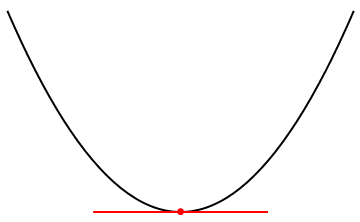
\includegraphics[width=\textwidth]{figures/cp01.png}
		\caption{$f'(c) = 0$,\\local minimum}
	\end{subfigure}
	\hfill
	\begin{subfigure}{0.3\textwidth}
		\centering
		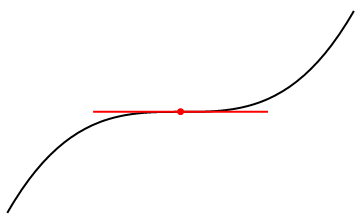
\includegraphics[width=\textwidth]{figures/cp02.png}
		\caption{$f'(c) = 0$,\\no local optimum}
	\end{subfigure}
	\hfill
	\begin{subfigure}{0.3\textwidth}
		\centering
		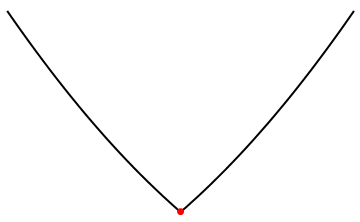
\includegraphics[width=\textwidth]{figures/cp03.png}
		\caption{$f'(c)$ undefined,\\local minimum}
	\end{subfigure}
	\\
	\begin{subfigure}{0.3\textwidth}
		\centering
		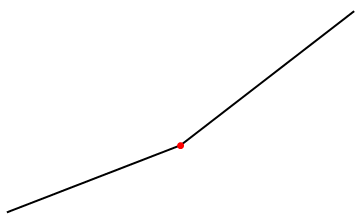
\includegraphics[width=\textwidth]{figures/cp04.png}
		\caption{$f'(c)$ undefined,\\no local optimum}
	\end{subfigure}
	\hfill
	\begin{subfigure}{0.3\textwidth}
		\centering
		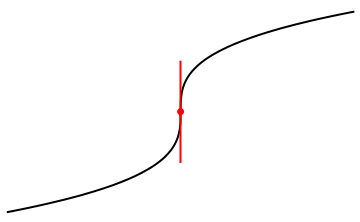
\includegraphics[width=\textwidth]{figures/cp05.png}
		\caption{$f'(c)$ undefined,\\no local optimum}
	\end{subfigure}
	\hfill
	\begin{subfigure}{0.3\textwidth}
		\centering
		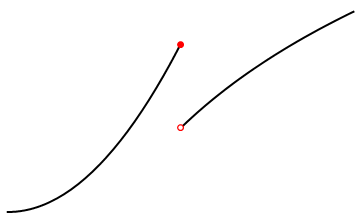
\includegraphics[width=\textwidth]{figures/cp06.png}
		\caption{$f'(c)$ undefined,\\local maximum}
	\end{subfigure}
	\\
	\begin{subfigure}{0.3\textwidth}
		\centering
		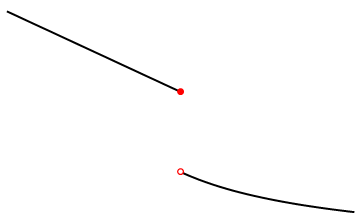
\includegraphics[width=\textwidth]{figures/cp07.png}
		\caption{$f'(c)$ undefined,\\no local optimum}
	\end{subfigure}
	\hfill
	\begin{subfigure}{0.3\textwidth}
		\centering
		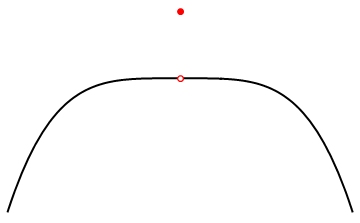
\includegraphics[width=\textwidth]{figures/cp08.png}
		\caption{$f'(c)$ undefined,\\local maximum}
	\end{subfigure}
	\hfill
	\begin{subfigure}{0.3\textwidth}
		\centering
		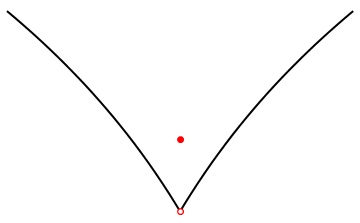
\includegraphics[width=\textwidth]{figures/cp09.png}
		\caption{$f'(c)$ undefined,\\local maximum}
	\end{subfigure}
	
	\caption{Examples of different types of critical point for a function $f : \mathbb{R} \to \mathbb{R}$.}
	\label{fig:critical}
\end{figure}

Critical numbers are used in Calculus~I to characterize candidates for local extrema. Since the local extrema of a function can only occur at critical points or the boundaries of an interval, we can search for the global minimum or maximum of an objective function by finding any and all critical points, checking their function values, checking the function values on the boundaries of the feasible set, and then simply picking the solution with the smallest or largest objective value.

All of this can be generalized in a straightforward way for functions of more than one variable. The intuition behind Fermat's Theorem is that a local optimum of a differentiable function $f(x)$ should be a stationary point of $f$, meaning that the instantaneous rate of change in $f$ with respect to $x$ should be zero, i.e.~$\frac{df}{dx} = 0$. For a function of two variables $f(x,y)$ we need for $f$ to be stationary with respect to \textit{both} $x$ \textit{and} $y$, which is true as long as $\frac{\partial f}{\partial x} = 0$ \textit{and} $\frac{\partial f}{\partial y} = 0$. More generally we require that all first-order partial derivatives of the function be zero simultaneously, which is equivalent to the gradient of the function being zero.

\newpage%%%

\begin{theorem}[Fermat's Theorem for Functions of Several Variables]
\label{thm:fermat2}
	Let $f : D \to \mathbb{R}$ be a real-valued function defined on an open set $D \subseteq \mathbb{R}^n$. If $\mathbf{c}$ is a local optimum of $f$ and $f$ is differentiable at $\mathbf{c}$, then $\nabla f(\mathbf{c}) = \mathbf{0}$.
\end{theorem}

Corollary~\ref{cor:fermat} also generalizes in a straightforward way.

\begin{corollary}
\label{cor:fermat2}
	Let $f : D \to \mathbb{R}$ be a real-valued function defined on some set $D \subseteq \mathbb{R}^n$. If $\mathbf{c}$ is a local optimum of $f$, then at least one of the following must be true:
	\begin{enumerate}[(a)]
		\item $\nabla f(\mathbf{c}) = \mathbf{0}$
		\item $\nabla f(\mathbf{c})$ is undefined
		\item $\mathbf{c}$ is on the boundary of $D$
	\end{enumerate}
\end{corollary}

This leads us to the definition of a \textit{critical point}, which is the multidimensional equivalent of the critical number.

\begin{definition}[Critical Point]
	Let $f : D \to \mathbb{R}$ be a real-valued function defined on an open set $D \subseteq \mathbb{R}^n$. A point $\mathbf{c} \in D$ is called a \textbf{critical point} of $f$ if $\nabla f(\mathbf{c})$ is either zero or undefined.
\end{definition}

Like with critical numbers, critical points can be used to characterize candidates for local extrema for functions of multiple variables, and they are used in the same way to solve simple optimization problems in Calculus~III. See Figure~\ref{fig:critical3d} for examples of local extrema for functions of two variables.

\begin{figure}[h]
	\centering
	
	\begin{subfigure}{0.3\textwidth}
		\centering
		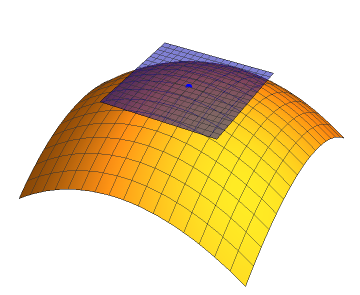
\includegraphics[width=\textwidth]{figures/cpsurf01.png}
		\caption{$\nabla f(\mathbf{c}) = \mathbf{0}$,\\local maximum}
	\end{subfigure}
	\hfill
	\begin{subfigure}{0.3\textwidth}
		\centering
		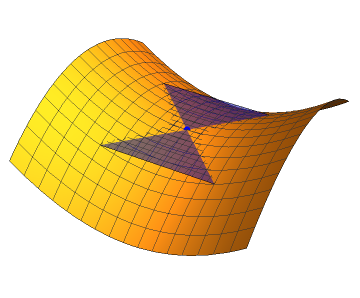
\includegraphics[width=\textwidth]{figures/cpsurf02.png}
		\caption{$\nabla f(\mathbf{c}) = \mathbf{0}$,\\no local optimum}
	\end{subfigure}
	\hfill
	\begin{subfigure}{0.3\textwidth}
		\centering
		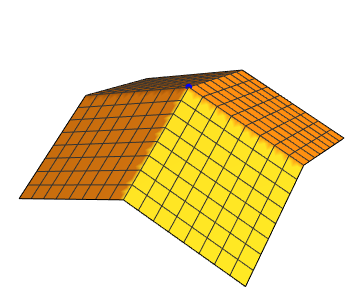
\includegraphics[width=\textwidth]{figures/cpsurf03.png}
		\caption{$\nabla f(\mathbf{c})$ undefined,\\local maximum}
	\end{subfigure}
	
	\caption{Examples of different types of critical point for a function $f : \mathbb{R}^2 \to \mathbb{R}$. The planes displayed in parts (a) and (b) are horizontal, and points on the surface parallel to them are points at which the gradient is zero.}
	\label{fig:critical3d}
\end{figure}

\newpage

%%%
\subsection{The Calculus Approach to Unconstrained Optimization}
\label{subsec:calculus}

The fact that the global optimum must also be locally optimal, and the characterization of local optima provided by Fermat's Theorem suggest a straightforward approach for solving simple unconstrained optimization problems:
\begin{enumerate}
	\item Find a way to express the optimization problem as a single, real-valued objective function. This may require using substitution to eliminate some constraints.
	\item Find any and all critical points of the objective function by doing the following:
	\begin{enumerate}
		\item Find its derivative (or gradient) and solve for any inputs that make it zero.
		\item Find its derivative (or gradient) and solve for any inputs that make it undefined. 
	\end{enumerate}
	\item List all critical points, as well as any points on the boundary of the feasible set. These are all candidates for local optima.
	\item Since the list is finite, simply check the objective value for each one. The largest of the objective values must be the global maximum, while the smallest must be the global minimum.
\end{enumerate}

It might help to review this procedure by going through a simple example from Calculus~I.

\begin{example}
\label{ex:calculus}
	Suppose we wish to design a rectangular enclosure divided into two equal halves. We have 3000~ft of fencing available, and we want the total area of the entire enclosure to be as large as possible. See Figure~\ref{fig:fence} for an illustration.
	
	\begin{figure}[h]
		\centering
		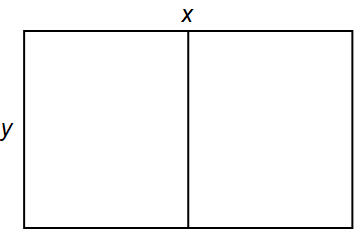
\includegraphics[width=0.3\textwidth]{figures/fence.png}
		\caption{A divided enclosure with dimensions of $x$ and $y$ (in feet).}
		\label{fig:fence}
	\end{figure}
	
	To introduce some decision variables, let $x$ and $y$ be the dimensions of the enclosure (in feet), with $y$ being the dimension parallel to the dividing wall. Our goal is to choose $x$ and $y$ to produce the maximum possible area while obeying the limited fencing constraint. Since the area of an $x$-by-$y$ rectangle is $xy$, and there are 2 segments of length $x$ and 3 segments of length $y$, we arrive at the optimization problem
	\begin{align*}
		\max \quad& xy \\
		\mathrm{s.t.} \quad& 2x + 3y \le 3000 \\
		& x,y \ge 0
	\end{align*}
	
	Clearly maximizing the area means that we should use as much fencing as is available, so this is equivalent to the simpler problem
	\begin{align*}
		\max \quad& xy \\
		\mathrm{s.t.} \quad& 2x + 3y = 3000
	\end{align*}
	
	\begin{figure}[h]
		\centering
		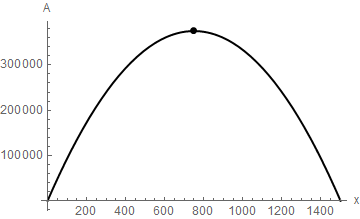
\includegraphics[width=0.3\textwidth]{figures/fence_calc1.png}
		\caption{The area of the fence as a function of only the dimension $x$. We can clearly see that the maximum area occurs at the stationary point at the vertex of the parabola.}
		\label{fig:fenceopt1}
	\end{figure}
	
	In order to solve this using the methods available in Calculus~I, we need to reduce this problem to an unconstrained optimization problem of a single variable. We can do that by applying the equality constraint $2x + 3y = 3000$ to solve for one of the variables in terms of the other, say $y = 1000 - \frac{2}{3} x$. Making this substitution leaves us with
	\begin{align*}
		\max \quad& x \left( 1000 - \frac{2}{3} x \right)
	\end{align*}
	which is something that \textit{can} be solved by the methods described above (see Figure~\ref{fig:fenceopt1}). In particular, we find the derivative of the objective $f(x) = 1000x - \frac{2}{3} x^2$ as
	\begin{align*}
		f'(x) = 1000 - \frac{4}{3} x
	\end{align*}
	
	This is always defined for all $x$, and setting it equal to zero leads to exactly one critical number: $x = 750$. Plugging this back into the $y$ equation gives a corresponding dimension of $y = 500$. The only other candidate optima occur on the boundaries of the feasible set, where $x = 0$ or $y = 0$, but since both of those result in an area of zero they represent the global minima, not the global maximum. We conclude that the optimal dimensions are $x = 750$~ft, $y = 500$~ft, for a total area of $375,\!000$~ft$^2$.
\end{example}

This is the general technique for solving simple optimization problems presented in Calculus~I and~III, and we should take a moment to appreciate how nice and unexpected of a result it is. Looking at the statement of a typical optimization problem, it isn't immediately obvious how to solve it. However, a bit of theoretical work allows us to find necessary conditions for optimality that concern the derivative (or gradient) of the objective function, which allows us to look for candidate solutions by simply solving an equation. This kind of result, wherein we can solve a difficult problem just by solving an equation, is pretty rare and valuable in applied mathematics.

However, even within Calculus~III, this approach is not enough for solving problems with more complicated sets of constraints. Fortunately the concept of \textit{stationarity} being necessary for optimality can be extended to work for constrained optimization in the form of \textit{Lagrange multipliers}.

%%%
\subsection{Lagrange Multipliers}
\label{subsec:lagrange}

The concept of critical points is enough to solve simple unconstrained optimization problems, as well as constrained optimization problems with very simple feasible sets (e.g.~sets defined by box constraints like $a \le x \le b, \, c \le y \le d$). For systems with more complicated sets of constraints, more sophisticated tools are required. For example, consider the constrained optimization problem
\begin{align*}
	\min \quad& x + y \\
	\mathrm{s.t.} \quad& x^2 + y^2 \le 1
\end{align*}
whose feasible set is the unit disk in $\mathbb{R}^2$ (see Figure~\ref{fig:constrainedopt}). The objective is differentiable and has a constant gradient $\nabla (x+y) = (1,1)$, which is clearly never zero, so there are no critical points. However, the feasible set is closed and bounded, so by the Extreme Value Theorem there must be a finite minimum value, and by Corollary~\ref{cor:fermat2} it must be somewhere on the boundary of the unit disk (i.e.~the unit circle $x^2 + y^2 = 1$). It isn't immediately obvious how to search for local extrema on this set, but Calculus~III provides an answer in the form of \textit{Lagrange multipliers}.

\begin{figure}[h]
	\centering
	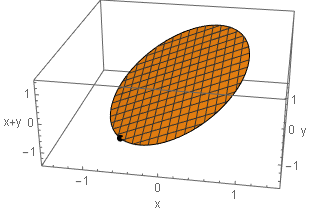
\includegraphics[width=0.4\textwidth]{figures/constrainedopt01.png}
	\caption{The surface $z = x+y$ (or possibly a waffle) plotted over the feasible set $x^2 + y^2 \le 1$. Our goal is to find the point at which $x+y$ is minimized, meaning the lowest point on this surface, which we can clearly see occurs on the boundary.}
	\label{fig:constrainedopt}
\end{figure}

\begin{theorem}[The Lagrange Multiplier Theorem]
\label{thm:lagrange}
	Let $f : D \to \mathbb{R}$ and $g : D \to \mathbb{R}$ be functions with continuous first partial derivatives on some open set $D \subseteq \mathbb{R}^n$ containing the smooth curve $g(\mathbf{x}) = 0$. Let $\mathbf{x^{\boldsymbol{*}}}$ be a locally optimal solution to the constrained optimization problem
	\begin{align*}
		\min \quad& f(\mathbf{x}) \\
		\mathrm{s.t.} \quad& g(\mathbf{x}) = 0
	\end{align*}
	
	Then there exists a unique number $\lambda \in \mathbb{R}$, called a \textbf{Lagrange multiplier}, such that
	\begin{align*}
		\nabla f(\mathbf{x^{\boldsymbol{*}}}) = \lambda \nabla g(\mathbf{x^{\boldsymbol{*}}})
	\end{align*}
\end{theorem}

Proving the Lagrange Multiplier Theorem is beyond the scope of this course\footnote{The proof of this theorem involves the use of the multivariate Chain Rule and the parameterizations of space curves. See an undergraduate Calculus~III textbook~\cite{stewart,openstax3} for details.}, but it has a few useful implications and extensions. For practical purposes, within Calculus~III, the Lagrange Multiplier Theorem is used to justify the \textbf{Method of Lagrange Multipliers} for solving simple constrained optimization problems. To be more precise, given a constrained optimization problem with a single equality constraint of the form
\begin{alignat*}{3}
	\min \quad& f(\mathbf{x}) &\qquad \text{or} \qquad&& \max \quad& f(\mathbf{x}) \\
	\mathrm{s.t.} \quad& g(\mathbf{x}) = 0 &&& \mathrm{s.t.} \quad& g(\mathbf{x}) = 0
\end{alignat*}
we can look for candidate solutions by solving the system
\begin{align}
	\label{eqn:lagrange1} \nabla f(\mathbf{x}) &= \lambda \nabla g(\mathbf{x}) \\
	\label{eqn:lagrange2} g(\mathbf{x}) &= 0
\end{align}

This is a system of $n+1$ equations (the $n$ components of the gradient vectors plus one additional equality constraint) and $n+1$ variables (the $n$ variables of $\mathbf{x}$ plus one additional variable $\lambda$). In general the system has finitely many solutions, so to solve the original optimization problem we can simply evaluate the objective function~$f$ at each solution~$\mathbf{x}$ and then pick the solution with either the smallest or the largest objective value. Equations~(\ref{eqn:lagrange1}) are the \textit{stationarity} conditions, and ensure that the solution meets the necessary condition for local optimality provided by the Lagrange Multiplier Theorem, while equation~(\ref{eqn:lagrange2}) is the \textit{feasibility} condition, which ensures that the solution is also guaranteed to be feasible.

\begin{example}
\label{ex:lagrange}
	Suppose we wish to solve the constrained optimization problem
	\begin{align*}
		\min \quad& x + y \\
		\mathrm{s.t.} \quad& x^2 + y^2 \le 1
	\end{align*}
	
	See Figure~\ref{fig:constrainedopt} for an illustration. As noted earlier, the gradient of the objective is defined and nonzero for all $(x,y)$, so there are no critical points within the unit disk. The global minimum must then lie on the boundary of the unit disk, which is equivalent to solving
	\begin{align*}
		\min \quad& x + y \\
		\mathrm{s.t.} \quad& x^2 + y^2 = 1
	\end{align*}
	
	Applying the Method of Lagrange Multipliers to this example, the system~(\ref{eqn:lagrange1})--(\ref{eqn:lagrange2}) is
	\begin{align*}
		1 &= 2x \lambda \\
		1 &= 2y \lambda \\
		x^2 + y^2 &= 1
	\end{align*}
	
	This is a system of three equations and three unknowns, and it has exactly two solutions: $(x,y,\lambda) = (-\frac{\sqrt{2}}{2}, -\frac{\sqrt{2}}{2}, -\frac{\sqrt{2}}{2})$ and $(x,y,\lambda) = (\frac{\sqrt{2}}{2}, \frac{\sqrt{2}}{2}, \frac{\sqrt{2}}{2})$. Since our goal is to minimize the objective $x+y$ we pick the first solution, therefore the optimal solution is $(x,y) = (-\frac{\sqrt{2}}{2}, -\frac{\sqrt{2}}{2})$ with an objective value of $-\sqrt{2}$.
\end{example}

It should be noted that the Method of Lagrange Multipliers could have also been used to solve Example~\ref{ex:calculus} without needing to first eliminate any variables.

\begin{example}
\label{ex:calculusalt}
	
	Given the same setup as Example~\ref{ex:calculus}, our goal is to solve the constrained optimization problem
	\begin{align*}
		\max \quad& xy \\
		\mathrm{s.t.} \quad& 2x + 3y = 3000
	\end{align*}
	
	\begin{figure}[h]
		\centering
		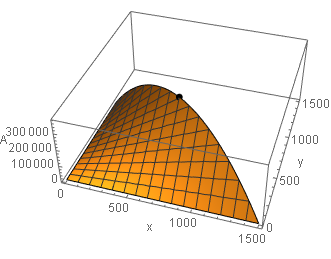
\includegraphics[width=0.4\textwidth]{figures/constrainedopt02.png}
		\caption{The surface $z = xy$ plotted over the feasible set $2x + 3y \le 3000$. Our goal is to find the point at which $xy$ is maximized, meaning the highest point on this surface.}
		\label{fig:calculusalt}
	\end{figure}
	
	See Figure~\ref{fig:calculusalt} for an illustration. Applying the Method of Lagrange Multipliers, the system~\mbox{(\ref{eqn:lagrange1})--(\ref{eqn:lagrange2})} is
	\begin{align*}
		y &= 2 \lambda \\
		x &= 3 \lambda \\
		2x + 3y &= 3000
	\end{align*}
	which has exactly one solution, $(x,y,\lambda) = (750,500,250)$, thus producing the same solution $x = 750$, $y = 500$ as before.
\end{example}

The Method of Lagrange Multipliers can be easily extended to handle problems with more than one equality constraint. Given a constrained optimization problem with $m$ equality constraints of the form
\begin{alignat*}{3}
	\min \quad& f(\mathbf{x}) &\qquad \iff \qquad&& \min \quad& f(\mathbf{x}) \\
	\mathrm{s.t.} \quad& \mathbf{g}(\mathbf{x}) = \mathbf{0} &&& \mathrm{s.t.} \quad& g_i(\mathbf{x}) = 0, \, i=1,2,\dots,m
\end{alignat*}
we introduce a separate Lagrange multiplier $\lambda_i$ for each constraint $g_i(\mathbf{x}) = 0$, $i=1,2,\dots,m$, and the necessary conditions for optimality become
\begin{alignat}{3}
	\label{eqn:lagrange3} \nabla f(\mathbf{x}) &= \boldsymbol{\lambda}^T \nabla \mathbf{g}(\mathbf{x}) &\qquad \iff \qquad&& \nabla f(\mathbf{x}) &= \sum_{i=1}^m \lambda_i \nabla g_i(\mathbf{x}) \\
	\label{eqn:lagrange4} \mathbf{g}(\mathbf{x}) &= \mathbf{0} &&& g_i(\mathbf{x}) &= 0, \, i=1,2,\dots,m
\end{alignat}
where $\boldsymbol{\lambda}^T$ represents the transpose of $\boldsymbol{\lambda}$.

The Method of Lagrange Multipliers comes from a more general approach to optimization called \textit{Lagrangian relaxation}, which we will discuss in more detail later in the course. Lagrangian relaxation is an important technique in certain branches of nonlinear optimization, and it is of central importance in \textit{duality theory}, which we will discuss in much more detail during our coverage of linear optimization. See Appendix~\ref{app:penalty} for a brief preliminary explanation of how to interpret what the Lagrange multipliers actually mean and where they come from.

Finally, we should note that the Method of Lagrange Multipliers applies \textit{only} when all constraints are \textit{equalities} rather than \textit{inequalities}. There is a generalization of Lagrange multipliers known as the \textit{Karush-Kuhn-Tucker (KKT) conditions} that works for inequality constraints, as well, which we may discuss near the end of the course depending on time. 

\newpage
%==============================================================================
\section{Practical Approaches to Optimization}
\label{sec:approaches}

To summarize the Calculus approach to optimization, Fermat's Theorem and the Method of Lagrange Multipliers both provide a way to characterize candidate optima by specifying conditions that must necessarily be true at a local optimum. In both cases the end result is a set of equations that can be solved to find local optima, after which we can simply check each the objective value at each local optimum to find which has the best objective value. Collectively, the Calculus-based methods fit the general format:

\textit{\textbf{Solving an Optimization Problem Analytically:} Find a system of equations that any optimal solution must theoretically satisfy, and solve that system explicitly to find (candidates for) the optima.}

This approach is simple and elegant, which is why it's a shame that it's almost never usable in practice. The example problems that you're used to from Calculus were all extremely simplistic and contrived in order to be solvable by hand, but in the real world we typically deal with very large problems (often with hundreds or thousands of variables and constraints) and problems whose objective and constraint functions are very complicated. Even if we could explicitly write down a system of equations of the form
\begin{align*}
	\nabla f(\mathbf{x}) = \mathbf{0}
\end{align*}
as with Fermat's Theorem or
\begin{align*}
	\nabla f(\mathbf{x}) &= \boldsymbol{\lambda}^T \nabla \mathbf{g}(\mathbf{x}) \\
	\mathbf{g}(\mathbf{x}) &= \mathbf{0}
\end{align*}
as with the Method of Lagrange Multipliers, for most real-world applications the resulting system would be so large and so nonlinear that it would be either extremely difficult or literally impossible to solve it analytically. However, even if we cannot directly apply the conclusions of the Calculus-based analytical methods, we can still apply the basic ideas the lead to them in the first place.

In this final section we will give a brief preview of some of the more practical approaches to optimization that we will be developing later in the course. For simplicity we will restrict our discussion to the case of the unconstrained minimization of a differentiable function $f$.

%%%
\subsection{Iterative Optimization Algorithms}
\label{subsec:iterative}

Fermat's Theorem implies that a local minimum can only occur where the derivative (or gradient) of the objective is zero. This is the \textit{stationarity} condition, and the logic behind it was that, if $f'(c)$ is nonzero at some input $c$, then we could either increase or decrease its input to achieve an even smaller objective value. In short, $f'(c)$ being nonzero means that the graph of $f$ has a nonzero slope at $c$, in which case we can move in the ``downhill'' direction to decrease the objective value. This idea of a nonzero slope indicating that we could move in the downhill direction extends to functions of several variables, since the negative gradient vector is always a direction in which $f$ decreases. This observation gives rise to a new strategy for finding a local minimum:

\textit{\textbf{Solving an Optimization Problem Iteratively:} Instead of trying to set up a system of equations to explicitly solve for a local minimum, we can instead just start with some initial guess and check the gradient of $f$ there. If the gradient is zero, then we've found a critical point, and if not, we can take a small step in the direction of decrease to achieve a better objective value. If we keep repeating the process until the gradient is close enough to zero, then we must end up at a local minimum.}

There are a few drawbacks to this type of iterative method. For one, it can only provide an approximate solution, but in most real-world applications that's fine. More importantly it only provides a way to find a \textit{local} minimum, not necessarily the \textit{global} minimum, since unlike the analytical approach it cannot enumerate every possible critical point. Unfortunately there is no good solution to that problem, but there are some heuristics that can be used in practice to try to find more than just one local minimum (repeatedly restarting the algorithm with a different random initial guess is one simple idea). In addition, if the objective happens to be convex, then finding a local minimum is sufficient for finding the global minimum.

We can describe this basic iterative approach more precisely by describing it as an algorithm:
\begin{enumerate}
	\item Begin with some initial guess $\mathbf{x}_0$.
	\item Repeat the following for iterations $n=0,1,2,\dots$ until the magnitude of $\nabla f(\mathbf{x}_n)$ becomes small enough (or until reaching an iteration cutoff):
	\begin{enumerate}
		\item Find a direction in which $f$ decreases starting from point $\mathbf{x}_n$.
		\item Choose a step size.
		\item Take a step of the chosen step size in the chosen direction to arrive at a new solution~$\mathbf{x}_{n+1}$.
	\end{enumerate}
	\item Output the solution that achieved the smallest objective value.
\end{enumerate}

This algorithm is intentionally vague since every aspect of it can be handled in many different ways, but almost all computational optimization algorithms follow this general structure. Every major optimization algorithm we will discuss in this class, from the simplex algorithm for linear programming to the local search-based methods for integer programming to the families of gradient and Newton-like algorithms for nonlinear programming, is based on this fundamental idea: Start with an initial guess, iteratively take steps in a direction of objective decrease, and stop when the objective stops decreasing.

%%%
\subsection{A Preview of Gradient Descent}
\label{subsec:descent}

As a final preview to help to illustrate this iterative approach more concretely, let's take a look at a very simple version of an algorithm called \textbf{gradient descent}. Suppose we want to minimize a differentiable function $f : \mathbb{R}^n \to \mathbb{R}$ subject to no constraints. If $f$ is differentiable then $\nabla f(\mathbf{x})$ is defined everywhere, so we can use the gradient of $f$ to find a descent direction in each iteration. We might consider trying the algorithm:
\begin{enumerate}
	\item Begin with some initial guess $\mathbf{x}_0$.
	\item Repeat the following for iterations $n=0,1,2,\dots$ until the magnitude of $\nabla f(\mathbf{x}_n)$ becomes small enough (or until reaching an iteration cutoff):
	\begin{enumerate}
		\item Compute $\nabla f(\mathbf{x}_n)$.
		\item Update the solution by taking a step in the direction of $-\nabla f(\mathbf{x}_n)$, say
		\begin{align*}
			\mathbf{x}_{n+1} = \mathbf{x}_n - \nabla f(\mathbf{x}_n)
		\end{align*}
	\end{enumerate}
	\item Output the solution that achieved the smallest objective value.
\end{enumerate}

This type of iterative approach might remind you of \textit{Euler's method} for numerically solving ordinary differential equations, and the basic idea behind both is the same: We know which direction we should be moving in at each point, so we iteratively take small steps in those directions\footnote{In fact, gradient descent is equivalent to Euler's method applied to a system of differential equations of the form $\mathbf{x}'(t) = -\nabla f(\mathbf{x}(t))$, in which case a local minimum of $f$ corresponds to a steady state of the differential equations.}.

If you actually try implementing this algorithm to solve a specific nonlinear optimization problem, you might notice that it doesn't always work very well. In many instances it will produce a sequence of solutions that chaotically orbit around local minima without actually approaching them. We will discuss why this is later in the course, as well as some of the many refinements of gradient descent for dealing with additional complexities (for example, what to do if the gradient is difficult or impossible to compute, or what to do if the objective is non-differentiable, or what to do if constraints are present).

%==============================================================================

% Update bibliography with BibTeX
\bibliographystyle{abbrvnat}
\bibliography{references}

\appendix

\newpage
%==============================================================================
\section{Partial Derivatives and the Gradient Vector}
\label{app:partial}

Calculus~III is not technically a prerequisite for this course, but it includes a few important definitions that will be important for us later in the course, particularly during our coverage of nonlinear optimization. For that reason, we will briefly review the concept of the \textit{partial derivative} and the \textit{gradient vector}, both of which are extremely important in optimization. See Stewart's \textit{Calculus}~\cite{stewart} or OpenStax \textit{Calculus~3}~\cite{openstax3} for more details.

\begin{definition}[The Partial Derivative for Two Variables]
	Let $f : \mathbb{R}^2 \to \mathbb{R}$ be a function of two variables, $f(x,y)$. The \textbf{partial derivative} of $f$ with respect to $x$ is defined as
	\begin{align*}
		\frac{\partial f}{\partial x} := \lim_{h \to 0} \frac{f(x+h,y) - f(x,y)}{h}
	\end{align*}
	(provided the limit exists). Likewise, the partial derivative of~$f$ with respect to~$y$ is defined as
	\begin{align*}
		\frac{\partial f}{\partial y} := \lim_{h \to 0} \frac{f(x,y+h) - f(x,y)}{h}
	\end{align*}
	(provided the limit exists).
\end{definition}

The partial derivative is a generalization of the \textit{ordinary derivative} from Calculus~I, which is defined only for functions of single variables. The~$\partial$ symbol is a curly~$d$ to distinguish the partial derivative from the ordinary derivative\footnote{Later in the course we will see that the~$\partial$ symbol is also commonly used to denote some other things, like the \textit{subgradient} of a function and the boundary of a region. As always, context should make it clear which meaning is intended.}. This definition extends to functions of more than two variables in a straightforward way. Like the ordinary derivative the partial derivative is defined as a limit of difference quotients, and represents an \textit{instantaneous rate of change}, but now with respect to just one of several input variables. For example, $\frac{\partial}{\partial x} f(x,y)$ represents the instantaneous rate of change in $f$ as $x$ increases while $y$ remains constant, while $\frac{\partial}{\partial y} f(x,y)$ represents the instantaneous rate of change in $f$ as $y$ increases while $x$ remains constant.

Evaluating partial derivatives is quite straightforward (assuming we have a simple, closed-form definition for our function), and the method for doing so comes directly from the definition. To find the partial derivative of a function with respect to a particular variable, simply apply the usual differentiation rules from Calculus~I, but treat all other variables as constant. For example, given a function
\begin{align}
	\label{eqn:exmultivariate} u(x,y,z) = x^2 y + 4y - x \sin z
\end{align}
its partial derivatives are
\begin{align*}
	\frac{\partial}{\partial x} u(x,y,z) &= 2xy - \sin z \\
	\frac{\partial}{\partial y} u(x,y,z) &= x^2 + 4 \\
	\frac{\partial}{\partial z} u(x,y,z) &= -x \cos z
\end{align*}

Notice that the partial derivative with respect to one variable is, in general, an expression that depends on \textit{all variables}, which makes sense. How quickly a function's value increases as one input is increased generally depends on the current values of all inputs, not just the one being increased.

The partial derivative can be used to define something called the \textit{gradient vector}, which is a concept of central importance in optimization.

\begin{definition}[The Gradient Vector for Two Variables]
	Let $f : \mathbb{R}^2 \to \mathbb{R}$ be a function of two variables, $f(x,y)$, with continuous first partial derivatives. The \textbf{gradient} of $f$ is a vector defined as
	\begin{align*}
		\nabla f(x,y) := \begin{bmatrix}
			\displaystyle \frac{\partial f}{\partial x} \\ \\
			\displaystyle \frac{\partial f}{\partial y}
		\end{bmatrix}
	\end{align*}
\end{definition}

This definition generalizes in a straightforward way to functions of more than two variables. In general, the gradient of a function $f : \mathbb{R}^n \to \mathbb{R}$ is a vector $\nabla f(\mathbf{x}) \in \mathbb{R}^n$ consisting of all partial derivatives of~$f$ with respect to all~$n$ of its inputs, in order. The $\nabla$ symbol is called a ``nabla'', and when treated as a differential operator is is called the ``gradient operator'' or the ``del operator''.

Sometimes a subscript is added to the nabla symbol to clarify which partial derivatives should be included, which may be useful for expressions that involve many variables. For example, given the function $u$ defined in~(\ref{eqn:exmultivariate}) above,
\begin{align*}
	\nabla u(x,y,z) = \begin{bmatrix}
		2xy - \sin z \\
		x^2 + 4 \\
		-x \cos z
	\end{bmatrix}
\end{align*}
which includes all three partial derivatives of $u$, in order, while
\begin{align*}
	\nabla_{x,y} u(x,y,z) = \begin{bmatrix}
		2xy - \sin z \\
		x^2 + 4
	\end{bmatrix}
\end{align*}
which includes only the partial derivatives of $u$ with respect to $x$ and $y$, not $z$.

The gradient vector has a number of important applications in optimization, and is used both for characterizing critical points and for defining ascent/descent directions in iterative algorithms. In general it can be thought of as the multidimensional equivalent of the ordinary derivative, and it often appears in place of the ordinary derivative when we generalize one-dimensional optimization results or algorithms to more than one dimension.

For example, for a function $f : \mathbb{R} \to \mathbb{R}$ of a single variable $f(x)$, a \textit{critical number} (which is a candidate for being a local optimum) is defined as being a value $x^*$ for which $\frac{d}{dx} f(x^*)$ is either~$0$ or undefined. For a function $f : \mathbb{R}^n \to \mathbb{R}$ of multiple variables $f(\mathbf{x})$, a critical point is a point $\mathbf{x^{\boldsymbol{*}}}$ for which $\nabla f(\mathbf{x^{\boldsymbol{*}}})$ is either~$\mathbf{0}$ or undefined. Moreover, in the same way that the sign of the ordinary derivative indicates the direction of ascent, the direction of the gradient vector also indicates the direction of ascent.

More specifically, for a function $f : \mathbb{R} \to \mathbb{R}$ of a single variable $f(x)$ and a particular solution~$x_0$, if we know that $\frac{d}{dx} f(x_0) > 0$ then we can say that increasing $x_0$ will increase the objective value, while if \mbox{$\frac{d}{dx} f(x_0) < 0$} we can say that decreasing $x_0$ will increase the objective value, and the magnitude $|\frac{d}{dx} f(x_0)|$ describes how quickly the objective value will increase. Likewise, for a function $f : \mathbb{R}^n \to \mathbb{R}$ of multiple variables $f(\mathbf{x})$ and a particular solution $\mathbf{x}_0$, moving in the direction of $\nabla f(\mathbf{x}_0)$ will always increase the objective value, moving in the opposite direction $-\nabla f(\mathbf{x}_0)$ will decrease it, and the magnitude $\|\nabla f(\mathbf{x}_0)\|$ describes how quickly the objective value will increase\footnote{To be more precise, the direction of $\nabla f(\mathbf{x})$ is the direction in which the \textit{directional derivative} of $f$ is maximized, while its magnitude is the maximum value of the directional derivative. See an undergraduate Calculus~III textbook~\mbox{\cite{stewart,openstax3}} for details.}. In short, we often say that $\nabla f(\mathbf{x})$ provides the \textit{direction of steepest ascent}, while its negative $-\nabla f(\mathbf{x})$ provides the \textit{direction of steepest descent}.

\newpage
%==============================================================================
\section{Lagrange Multipliers as Penalty Costs}
\label{app:penalty}

Before we begin our coverage of duality theory as it relates to linear optimization it will be useful to have a quick, intuitive idea for what Lagrangian Relaxation means and why it might work. Starting from a constrained minimization problem of the form
\begin{align}
	\label{eqn:relaxation1} \min \quad& f(\mathbf{x}) \\
	\label{eqn:relaxation2} \mathrm{s.t.} \quad& g(\mathbf{x}) = 0
\end{align}
it might not be immediately obvious how we should approach solving it. Unconstrained optimization is relatively easy (using, for example, the basic Calculus techniques discussed in Section~\ref{subsec:calculus}), so one idea that might occur to us would be to simply ignore the constraint to create something known as a \textit{relaxation} of the original problem
\begin{align*}
	\min \quad& f(\mathbf{x})
\end{align*}

This problem is much easier to solve than the original, but doing so might not be very useful for us since the unconstrained optimal solution might be nowhere near the constrained optimal solution. As a compromise between the two approaches, we might consider incorporating the constraint into the objective as a \textit{penalty cost} of the form
\begin{align}
	\label{eqn:relaxation3} \min \quad& f(\mathbf{x}) + \lambda \, g(\mathbf{x})
\end{align}
where $\lambda$ is a \textit{unit penalty cost} that we get to choose.

To explain, suppose that the optimal solution to the unconstrained problem results in a value of $g(\mathbf{x})$ much greater than $0$. Regardless of how low of an objective value $f(\mathbf{x})$ this solution achieves, we want to have $g(\mathbf{x}) = 0$ in order to maintain feasibility, so we would like to discourage ourselves from picking solutions that produce very large values of $g(\mathbf{x})$. By including a term of the form $\lambda \, g(\mathbf{x})$ in the objective, and by choosing $\lambda > 0$, we can penalize highly infeasible solutions by artificially increasing their objective values to make them less attractive. Likewise, if $g(\mathbf{x})$ is much less than $0$, choosing $\lambda < 0$ penalizes such infeasible solutions. The specific choice of $\lambda$ allows us to choose how much to penalize infeasible solutions, and whether to penalize solutions for which the $g(\mathbf{x})$ is either too large or too small.

Different choices of $\lambda$ result in the relaxed problem~(\ref{eqn:relaxation3}) having different optimal solutions. If we consider \textit{both} the decision variables~$\mathbf{x}$ \textit{and} the penalty costs~$\lambda$ to be variables under our control, we can see intuitively that a necessary condition for optimality is for the relaxed objective $f(\mathbf{x}) + \lambda \, g(\mathbf{x})$ to be stationary with respect to \textit{both}~$\mathbf{x}$ \textit{and}~$\lambda$. It should be stationary with respect to~$\mathbf{x}$ for the same reasons as discussed in Section~\ref{subsec:calculus}, which come from Fermat's Theorem, but it should also be stationary with respect to~$\lambda$ since the only way for the value of $\lambda \, g(\mathbf{x})$ to remain constant as $\lambda$ changes is for $g(\mathbf{x})$ to be zero, which occurs exactly when $\mathbf{x}$ is feasible. In short, finding a stationary point $(\mathbf{x},\lambda)$ of the relaxed objective~(\ref{eqn:relaxation3}) is equivalent to finding a solution~$\mathbf{x}$ for which the objective~(\ref{eqn:relaxation1}) is stationary and the constraint~(\ref{eqn:relaxation2}) is satisfied.

We can also use this idea of the \textit{relaxed objective} to write the Method of Lagrange Multipliers more succinctly. As a way of generalizing the relaxed objective~(\ref{eqn:relaxation3}) to systems with~$m$ constraint functions~$\mathbf{g}(\mathbf{x}) = (g_1(\mathbf{x}),g_2(\mathbf{x}),\dots,g_m(\mathbf{x}))$ and their associated penalty costs~$\boldsymbol{\lambda} = (\lambda_1,\lambda_2,\dots,\lambda_m)$, we can define an expression called the \textbf{Lagrangian} as
\begin{align*}
	\mathcal{L}(\mathbf{x},\boldsymbol{\lambda}) := f(\mathbf{x}) + \boldsymbol{\lambda}^T \mathbf{g}(\mathbf{x}) = f(\mathbf{x}) + \sum_{i=1}^m \lambda_i g_i(\mathbf{x})
\end{align*}

The Lagrangian represents the relaxed objective, and is a function of both the decision variables~$\mathbf{x}$ and the unit penalty costs (which is what the Lagrange multipliers represent)~$\boldsymbol{\lambda}$. The system of equations~(\ref{eqn:lagrange3})--(\ref{eqn:lagrange4}) that define the Method of Lagrange Multipliers can then be written as simply
\begin{align}
	\label{eqn:lagrangian} \nabla_{\mathbf{x},\boldsymbol{\lambda}} \mathcal{L}(\mathbf{x},\boldsymbol{\lambda}) = \mathbf{0}
\end{align}

Based on the above discussion, solving~(\ref{eqn:lagrangian}) means finding a solution for which the relaxed objective is stationary. We can also see explicitly why this is equivalent to the Method of Lagrange Multipliers as defined in Section~\ref{subsec:lagrange}, since
\begin{align}
	\label{eqn:lagrangeblock} \nabla_{\mathbf{x},\boldsymbol{\lambda}} \mathcal{L}(\mathbf{x},\boldsymbol{\lambda}) = \begin{bmatrix}
		\nabla_{\mathbf{x}} \big( f(\mathbf{x}) + \boldsymbol{\lambda}^T \mathbf{g}(\mathbf{x}) \big) \\
		\nabla_{\boldsymbol{\lambda}} \big( f(\mathbf{x}) + \boldsymbol{\lambda}^T \mathbf{g}(\mathbf{x}) \big)
	\end{bmatrix} = \begin{bmatrix}
		\nabla_{\mathbf{x}} f(\mathbf{x}) + \boldsymbol{\lambda}^T \nabla_{\mathbf{x}} \mathbf{g}(\mathbf{x}) \\
		\mathbf{g}(\mathbf{x})
	\end{bmatrix}
\end{align}

Setting this equal to $\mathbf{0}$, the upper block portion of~(\ref{eqn:lagrangeblock}) is $\nabla_{\mathbf{x}} f(\mathbf{x}) + \boldsymbol{\lambda}^T \nabla_{\mathbf{x}} \mathbf{g}(\mathbf{x}) = \mathbf{0}$. This can be rearranged to become
\begin{align*}
	\nabla_{\mathbf{x}} f(\mathbf{x}) = -\boldsymbol{\lambda}^T \nabla_{\mathbf{x}} \mathbf{g}(\mathbf{x})
\end{align*}
which is equivalent to~(\ref{eqn:lagrange3}) with the signs of the Lagrange multipliers reversed. The lower block portion of~(\ref{eqn:lagrangeblock}) in turn is simply
\begin{align*}
	\mathbf{g}(\mathbf{x}) = \mathbf{0}
\end{align*}
which is exactly the feasibility condition~(\ref{eqn:lagrange4}). Therefore solving the system~(\ref{eqn:lagrangian}) for $\mathbf{x}$ is equivalent to solving the system~(\ref{eqn:lagrange3})--(\ref{eqn:lagrange4}) for $\mathbf{x}$. The two solutions will include Lagrange multipliers with opposite signs, but since the Lagrange multipliers aren't part of the original optimization problem we generally don't care about their specific values.

\end{document}
